F% PERFORMANCE METRICS ==========================================================
\section{Performance Metrics}
\label{appendix_metrics}

Examples are given below for explicitly calculating the performance metrics used in determining the quality of 3D bounding box (``bbox") predictions generated by the Stereo Point Cloud network (SPCLnet)

\subsection{Intersection Over Union}
Recall that IOU is critical in vision networks for determining whether a result is a true positive (TP) or a false positive (FP). To assist in understanding IOU, a code snippet as well as an example are presented. All aspects of calculating the IOU (including area and intersection) are broken up into multiple pieces, but presented together below. For n-dimensions, the code (presented here in python) is as follows:

\begin{figure}[ht]
\setstretch{0.84} % want code to be nice and compact
\begin{lstlisting}
import numpy as np
def extent(box,inclusive=False):
    o = 1 if(inclusive) else 0 # add '1' if inclusive is true
    b = np.array(box).reshape((2,-1)).T # now in internal convention
    return np.product([i[1]-i[0]+o for i in b])
def intersection(box1,box2,inclusive=False):
    o = 1 if(inclusive) else 0 # add '1' if inclusive is true
    b1=np.array(box1).reshape((2,-1)).T
    b2=np.array(box2).reshape((2,-1)).T # internal convention
    c=np.stack((b1,b2),2)
    # for each dimension, get (min(upperbound)-max(lowerbound)) and get product
    val=1
    for i in range(len(b1)):
        ans=np.min(c[i,1,:])-np.max(c[i,0,:])
        val*=max(ans,0) # if have negative dimension, have no intersection
    return val

def IOU(b1,b2,inclusive=False,criterion=-1):
    inter = intersection(b1,b2,inclusive)
    union = extent(b1,inclusive)+extent(b2,inclusive)-inter
    if(criterion==-1):
        return inter / union
    elif(criterion==0):
        return inter / extent(b1,inclusive)
    else:
        return inter / extent(b2,inclusive)

\end{lstlisting}
\onehalfspacing % set line spacing back to normal
\caption{Python implementation of generalized IOU calculation.}
\label{code_iou}
\end{figure}

\subsubsection{Example: IOU of a Ground Truth and Prediction Label}
\def \pxpx {\ [px^2]}
\def \Asub #1{A\textsubscript{#1}}

Suppose there is an image, as given below, where there is a ground truth label `gt' and a prediction label `pr' with 2D bounding boxes formatted as \texttt{[x1,y1,x2,y2]}, all units in pixels. To determine the IOU of the image, the calculations are listed below. Because boxes represent pixel values, remember to add ``1" to each dimension.

\begin{enumerate}\itemsep=-0.5em
    \item Find area of each bounding box: \\ $\Asub{gt} = (x2-x1+1)*(y2-y1+1) = 16,335 \pxpx $ , $ \Asub{pr} = 12905 \pxpx $
    \item Find overlapping area, e.g. intersection (see \ref{code_iou} for more info): $I = 11455 \pxpx $
    \item Calculate IOU: $\frac{I}{\Asub{gt} + \Asub{pr} - I} = 0.644 $
\end{enumerate}

\begin{figure}[H]
    \centering
    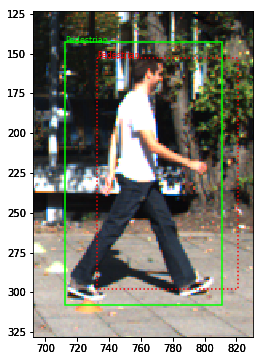
\includegraphics[width=.4\textwidth]{../media/iou_example.png}
    \caption{IOU calculation example. Ground truth (green solid) has BB: [712,143,810,307]. Prediction (red dotted) has BB: [732,153,820,297]. IOU is 0.644.}
    \label{iou_example}
\end{figure}


\subsection{Precision \& Recall}
Gathering all predictions together, one may then take the confidence score and outcome (TP, FP) of each prediction and create a precision-recall curve. To avoid extra steps regarding calculating a set of bounding boxes and determining IOU score, the following example uses a set of randomly generated outcomes values and confidence scores, listed below in Table \ref{precrecdat}.

\begin{table}[ht]
\centering
\caption{Precision-recall dummy data. Outcomes are either TP or FP, given as a `1' or `0', respectively. Confidence values are how confident the ``detection" was. In the true evaluation code, TP/FP is determined internally, and confidence values are the ``scores" in each detection label. Rows are conveniently given in order of descending confidence score.}
\footnotesize 
\begin{tabular}{|c|c|}%
\hline
\bfseries Outcomes & \bfseries Confidence % specify table head
\csvreader[head to column names]{../media/precrecdat.csv}{}% use head of csv as column names
{\\\hline\csvcoli&\csvcolii}% specify your columns here
\\\hline
\end{tabular}
\label{precrecdat}
\end{table}

The steps are as follow:
\begin{enumerate}\itemsep=-0.5em
    \item Begin with a confidence score vector and a outcomes vector
    \item Sort scores and corresponding outcomes by descending score value
    \item OPTIONAL: Identify unique index locations for approximate threshold indices (done in official code, not necessary)
    \item Create ``cumulative sum" TP-vector and FP vectors
    \item Calculate precision \& recall in vector form (unrefined)
    \item Refine precision vector $pr$ and \& recall vector $re$ (OPTIONAL: remove indices after TP vector stops increasing)
    \item OPTIONAL: Sort by descending recall value (done in official code, not necessary)
\end{enumerate}

\textbf{{\large Step 1: Obtain data}} \\
To begin, a randomly generated set of results (outcome and confidence scores) are given in Table \ref{precrecdat}. One may imagine that this table was generated after comparing car 3D bounding boxes against a set of ground truths and ensuring the IOU value was above a minimum threshold.

\textbf{{\large Step 2: Sort data by descending confidence score}} \\
In the case of this example, the values already sorted in this manner. Care must be taken to ensure that both a given result's confidence AND outcome (True or False) are kept in the same index location.
\begin{lstlisting}[numbers=left]
indices=np.argsort(ypred)[::-1]
ypred=ypred[indices]
ytrue=ytrue[indices]
\end{lstlisting}

\textbf{{\large Step 3 (OPTIONAL): Obtain indices of unique vectors}} \\
The purpose of this is to simply avoid needless calculation later, although empirically it has been found that the final graph and corresponding AP score are either identical or nearly so. This step WILL be carried out in this example, but may be omitted. Looking at the table, and assuming zero-based indexing as is typical in Python and other programming languages, the resulting vector is: $\texttt{[0,1,2,3,4,5,6,7,8,9,10,12,13,14,15,16,17,18]}$. Notice that index 11 and 19 are missing. ADDITIONALLY, the final index must be added to ensure that the graph terminates properly. If this step is not carried out, the correct value of the vector \texttt{threshold\_idxs} is generated instead via Line 5 below. To demonstrate the difference, please refer to Figure \ref{precrec_step3} below, and note that the AP value is still identical. In the vast majority of usage, the graph does indeed look identical.
\begin{lstlisting}[numbers=left]
if(get_unique_indices):
    distinct_value_indices = np.where(np.diff(conf))[0]
    threshold_idxs = np.append(distinct_value_indices,outcomes.size-1)
else:
    threshold_idxs = np.arange(conf.size) # sequence from 0 to N-1
\end{lstlisting}

\begin{figure}[H]
    \centering
    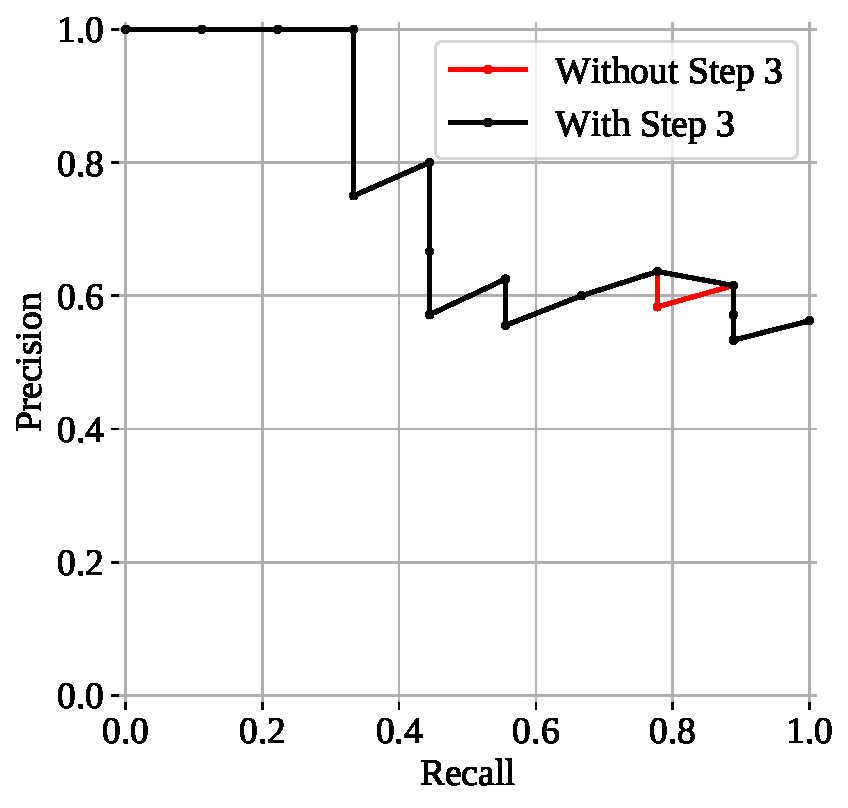
\includegraphics[width=0.45\linewidth]{../media/precrec_step3.pdf}
    \caption{Comparison of possible graph differences if Step 3 is skipped.}
    \label{precrec_step3}
\end{figure}


\textbf{{\large Step 4: Get Cumulative Sum for TP \& FP }} \\
The generation of an aggregate TP and FP vector enables precision and recall to be calculated as a vector as well, not only as scalar values. This is achieved by calculating the cumulative sum of the TP and FP arrays.
\begin{lstlisting}[numbers=left]
tps = np.cumsum(outcomes)[threshold_idxs]
fps = 1+threshold_idxs - tps
\end{lstlisting}


\textbf{{\large Step 5: Calculate Precision \& Recall}} \\
Precision and recall are calculated, but are still in a ``raw" form after this step. This means that there is some extra, unnecessary data as well as a theoretical point to be appended. As given by Equations \ref{eq_prec}, precision calculated, with some adaptation for code. Recall is often calculated differently than the theoretical form, here given as a division of the cumulative sum of true positive values by the final value.

\begin{lstlisting}[numbers=left]
precision = tps/(tps+fps)
precision[np.isnan(precision)]=0
recall = tps/tps[-1]
\end{lstlisting}


\textbf{{\large Step 6: Refine the data}} \\
Here, indices are removed after the cumulative sum of TP ceases to increase; additionally, artificial point at recall=0, precision=1 is added to the vectors (inserted at index 0). The first modification is optional, merely an aesthetic / time-saving choice, shown below in Figure \ref{precrec_step6}, but the artificial point is necessary for an accurate calculation of AP.

\begin{lstlisting}[numbers=left]
if(remove_extra_indices):
    lastind = tps.searchsorted(tps[-1])+1
else:
    lastind = -1
recall = np.append(0,recall[:lastind])
precision = np.append(1,precision[:lastind])
\end{lstlisting}

\begin{figure}[H]
    \centering
    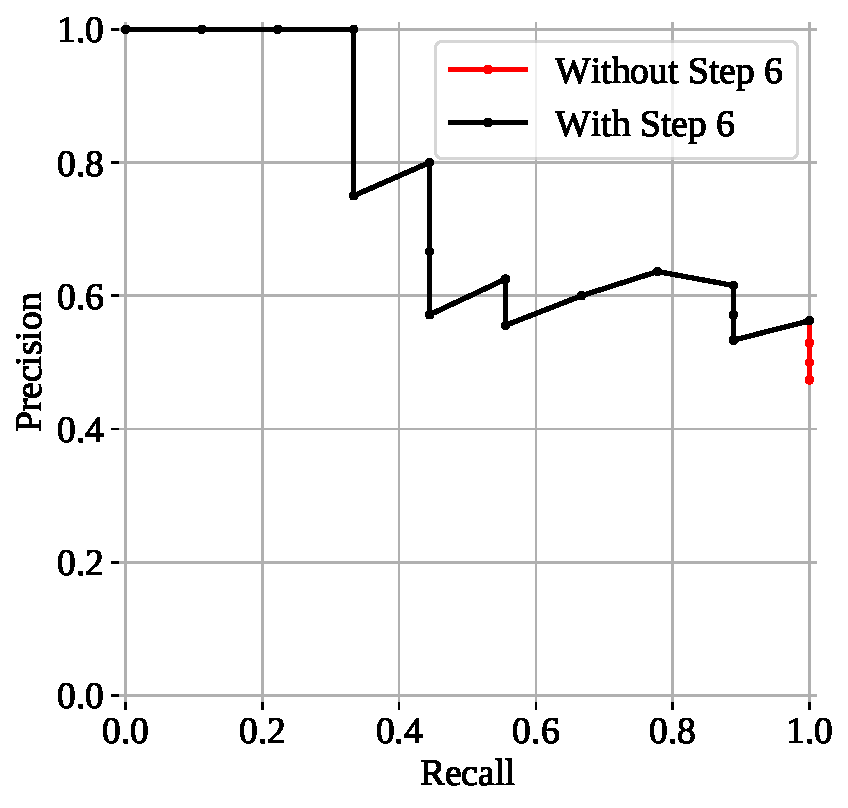
\includegraphics[width=0.45\linewidth]{../media/precrec_step6.pdf}
    \caption{Comparison of possible graph differences if Step 6 is skipped.}
    \label{precrec_step6}
\end{figure}

\textbf{{\large Step 7 (OPTIONAL): Sort by Descending Recall Value}} \\
This is an arbitrary step completed by the official matplotlib code, but may be carried out nonetheless if a certain convention is to be followed. It must be noted, however, that the proper calculation of AP requires the precision and recall vectors to be ordered by \textit{ascending} recall value.

\begin{lstlisting}[numbers=left]
recall=recall[::-1]
precision=precision[::-1]
\end{lstlisting}

Thus, the final values of precision and recall are calculated as given below in Table \ref{precrec_ans} and graphed in Figure \ref{precrec_steps}

\begin{figure}[H]
    \centering
    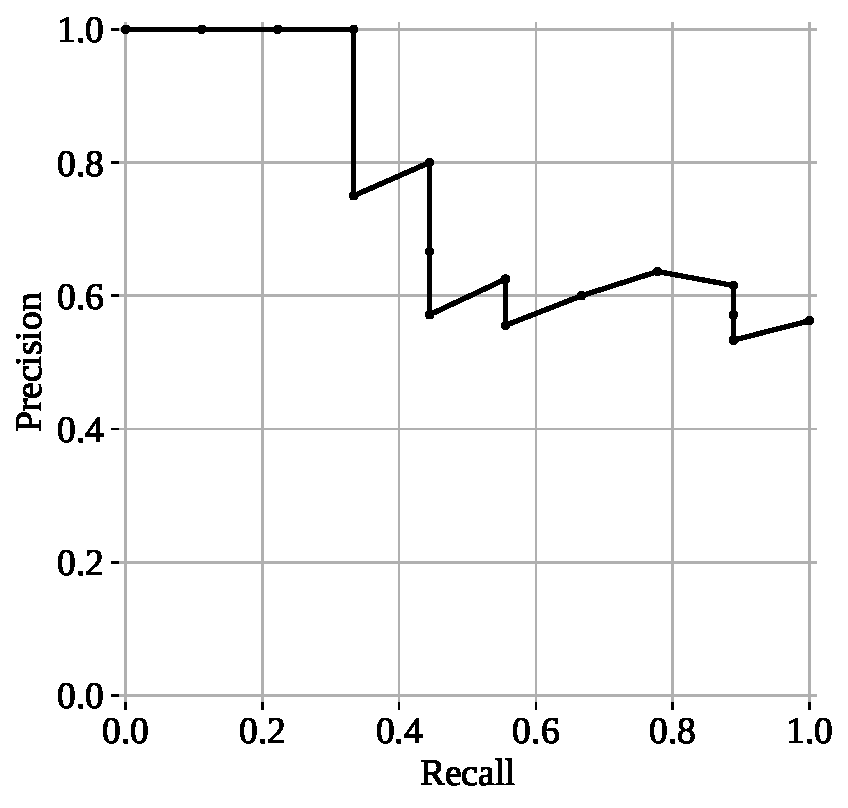
\includegraphics[width=0.4\linewidth]{../media/precrec_steps.pdf}
    \caption{Precision-recall curve if all steps are followed. Mathematically, AP value is same as without optional steps.}
    \label{precrec_steps}
\end{figure}

\begin{table}[H]
\centering
\caption{Precision-recall results, following all steps.}
\footnotesize 
\begin{tabular}{|c|c|}%
\hline
\bfseries Recall & \bfseries Precision % specify table head
\csvreader[head to column names]{../media/precrec_ans.csv}{}% use head of csv as column names
{\\\hline\csvcoli&\csvcolii}% specify your columns here
\\\hline
\end{tabular}
\label{precrec_ans}
\end{table}

\subsection{Calculating Average Precision}
To obtain the Average Precision from the previous example, simply follow Equation \ref{eq_ap}, or as implemented below (in a non-vectorized form). The AP of the values in Table \ref{precrec_ans} is 0.75992.

\begin{lstlisting}[numbers=left]
apsum=0
for i in range(0,len(precision)-1):
    print(i,end=' ')
    apsum+=(recall[i+1]-recall[i])*precision[i+1]
\end{lstlisting}






% ABOUT THE KITTI DATASET ======================================================
\newpage
\section{About the KITTI Dataset}
\label{appendix_kitti}

\subsection{Introduction}
To better understand the actual data that is being worked on, the KITTI dataset will be explained in-depth here. The acronym KITTI is a combination of ``KIT" (Karlsruhe Institute of Technology) and ``TTI" (Toyota Technical Institute, Chicago), the two cooperating institutions on the project. The very first thing to know about the KITTI dataset is that it is actually a set of datasets, each dataset specialized for some specific AI task. This means that there are some number of evaluation tasks / benchmarks, and a not-necessarily-unique dataset is used to enable completion of that task. The individual tasks are listed below with a brief description:

\begin{itemize}\itemsep=-0.5em
    \item Stereo, Optical Flow, Sceneflow (2012 \& 2015): An older (2012) and updated (2015) task comprised of 200 training and 200 test scenes. Each scene consists of a left and right image as well as a ``multi-view extension".
    \item Depth Completion / Estimation: A task comprised of about 93 thousand scenes containing RGB images and lidar scans.
    \item Visual Odometry / SLAM: 11 training and 11 testing stereo sequences with relevant grayscale, color, lidar, and ground truth poses.
    \item 2D / 3D / Bird's Eye View (BEV) Detection: 7481 training and 7518 test scenes with relevant color images, temporally preceding images, and lidar
    \item Single-/Multi- Object Tracking: An older (single) and in-development (multi) task consisting of multiple training and test sequences with relevant image, lidar, and GPS/IMU data.
    \item Road / Lane Detection: Around 289 training and 290 test images used for detecting various road scenes, containing image and lidar information.
    \item Semantic / Instance Segmentation: A task comprised of a set of stereo images like the Stereo task, but containing pixel-level localization of each class.
\end{itemize}

Each evaluation task also brings with it a ``dev kit" (a set of files that explain some of the technical information as well as helpful code), relevant camera / sensor calibration data of some kind, as well as some kind of ground truth label / file for each scene to assist with training. It should be noted that raw data of each dataset is available as well, but these are often unused and only kept as original source files for transparency. 

Each task is associated with one or more papers published by KIT and TTI, but these will not all be listed here. Instead, we shall now explain two datasets, especially the most relevant one: the KITTI object detection dataset, referred to as the KITTI dataset.

\subsection{The Stereo Dataset}
The stereo dataset, specifically 2015, will be briefly covered to describe its merits as well as why it presented overlap issues with the object detection dataset. What makes the stereo dataset important is that it is the dataset that was initially used to finetune the Pyramid Stereo Matching network and also the dataset used to help it achieve such a high position in the stereo benchmark.

The dataset itself is made up primarily of 200 training scenes and 200 testing scenes. The training scenes contain ground truth disparity maps, while the testing scenes do not and are used for final evaluation and submission to the benchmark website. For the project, only the training scenes were used. Each training scene is comprised of a left-hand side (LHS) color image, a RHS color image, a calibration file (containing transformation and other matrices), and a ground truth disparity file. There is also an available ``multi-view extension", containing 20 extra frames per scene, but this was not used. Figure \ref{stereo_sample} below shows all relevant data in a single sample scene: the left and right images, as well as a disparity map ground truth.

The ground truth labels were generated by a ``semi-automatic" process, as described by Menze and Geiger: the process was to ``extract disparity maps directly from the 3D information int he laser scans and fit geometrically accurate CAD models to moving 3D point clouds" \cite{menze_object_2015}. This explains several things about the ground truth disparity map in Figure \ref{stereo_sample}(c): the image is generally sparse, has no sample values above a certain horizontal line, and has a high density of pixels in the region where a car is outlined.

\begin{figure}[H]
    \centering
    \subfigure[left image]{
        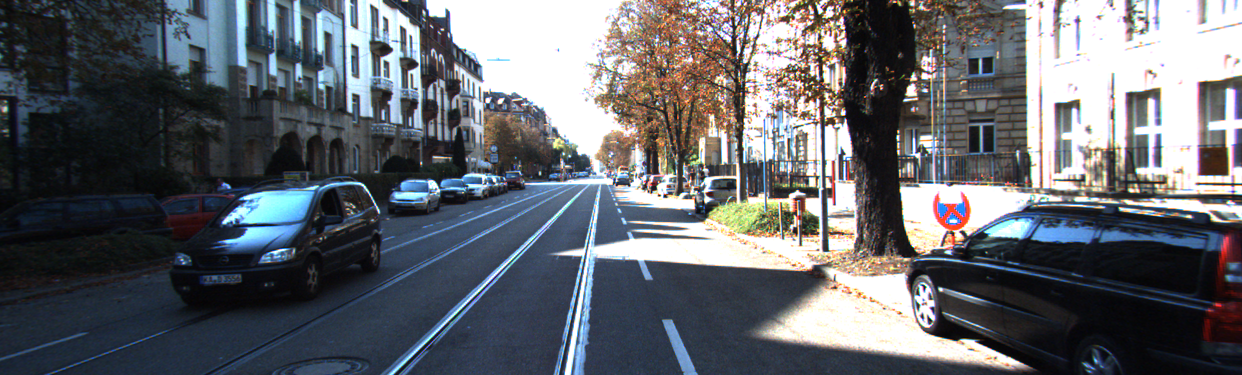
\includegraphics[width=0.487\linewidth]{../media/stereo_LHS_000000_10.png}}
    \subfigure[right image]{
        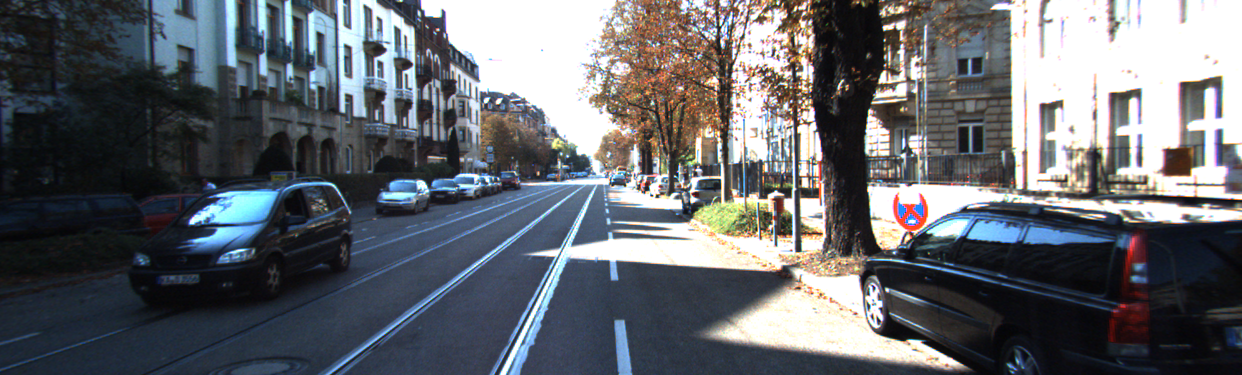
\includegraphics[width=0.487\linewidth]{../media/stereo_RHS_000000_10.png}}
    \subfigure[Ground truth disparity map. The value range for the original ground truth file may lie anywhere in the range of 1 to about 33,000.]{
        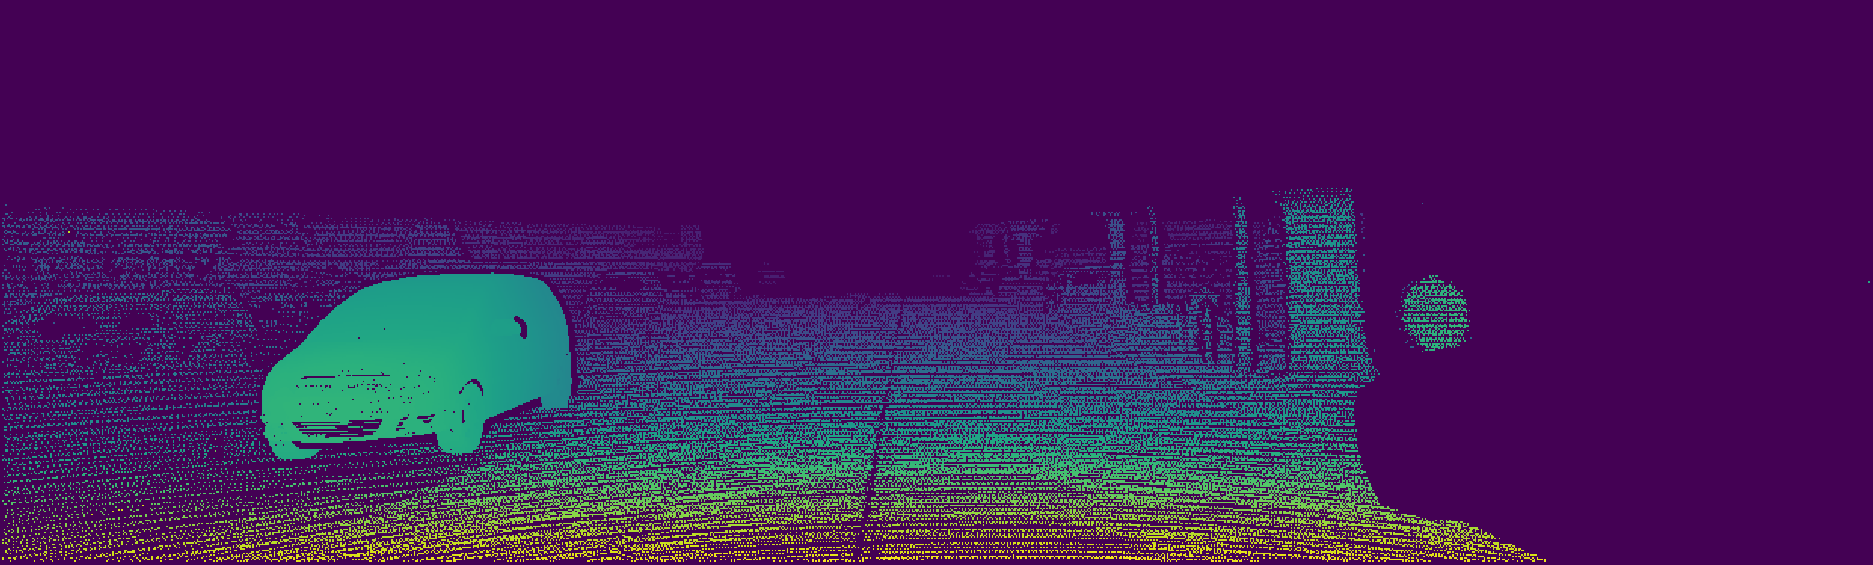
\includegraphics[width=1\linewidth]{../media/stereo_GTdisp_000000_10.png}}
    \caption{Sample scene from stereo dataset. Index 000000\_10}
    \label{stereo_sample}
\end{figure}



Ultimately, however, this dataset was not used for the primary reason described by \cite{wang_pseudo-lidar_2019}: there was an unacceptable amount of overlap, also known as data leakage, between the stereo dataset training data and the similar but unrelated object detection dataset. Figure \ref{similarity_stereo_objdet}, shown in Section 3, gives an example of a scene in the stereo dataset nearly matches a scene in the object detection dataset.

\subsection{The Object Detection Dataset \& Statistics}
The Object Detection dataset is the primary source of sensor data and media for this project, including PSMnet once it was determined that the stereo dataset had too much similarity with this dataset. This similarity could lead to data leakage, contaminating the integrity of the results. The Object Detection dataset is comprised of 7481 training scenes and 7518 testing scenes. The testing scenes were ignored for the purposes of this project, since they are unlabeled for KITTI benchmarking. Each scene in the training dataset contains a LHS (left-hand side) image, RHS image, lidar data, calibration data, and ground truth labels. An example of the images and lidar are given below in Figure \ref{objdet_sample}.

\begin{figure}[H]
    \centering
    \subfigure[LHS image]{
        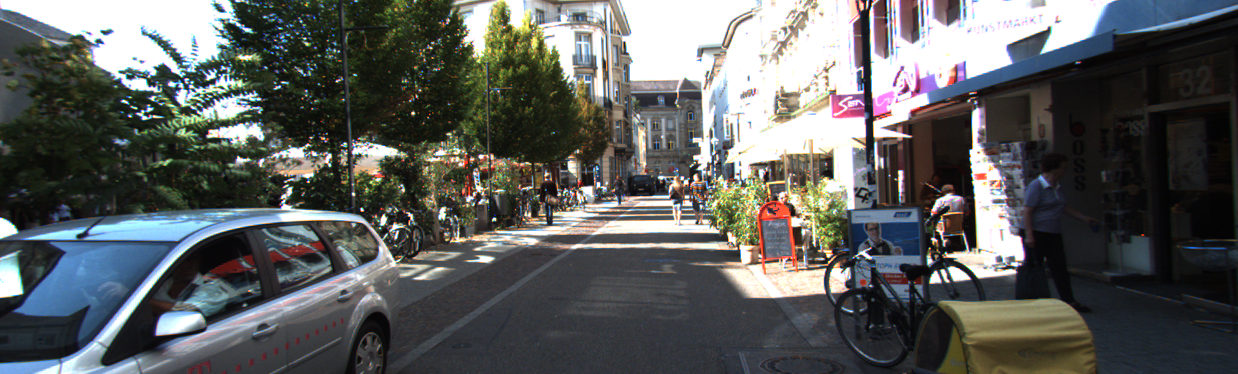
\includegraphics[width=0.487\linewidth]{../media/objdet_LHS_000015.png}}
    \subfigure[RHS image]{
        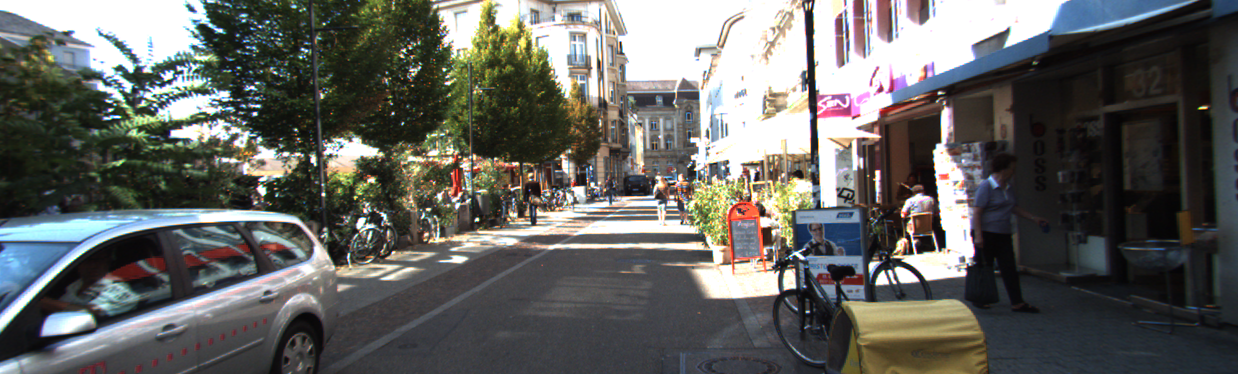
\includegraphics[width=0.487\linewidth]{../media/objdet_RHS_000015.png}}
    \subfigure[Velodyne lidar points projected onto image plane. Gray background for ease of viewing. Individual points use viridis colormap.]{
        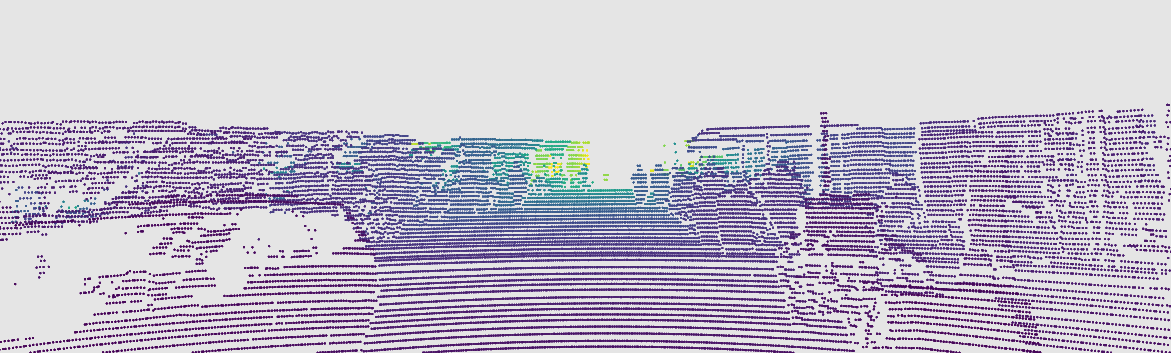
\includegraphics[width=1\linewidth]{../media/objdet_lidar_000015.png}}
    \caption{Sample scene from object detection dataset. Index 000015}
    \label{objdet_sample}
\end{figure}

In addition to the above lidar projection, the point cloud may be better visualized with an isometric view, rather than one from the camera's perspective. This is provided below. As is immediately obvious in Figure \ref{objdet_lidar_sample} and from knowledge of the hardware itself, a lidar scan is capable of capturing points surrounding the sensor in a 360\deg horizontal view. However, because of the nature of a typical color camera, points that are outside the camera's field of view are filtered out.

Another key piece of the object detection dataset is the label data. Ground truth labels are simply lines of text that contain an array of information about each instance of an object in the scene. An example label with value names is given below in Table \ref{kitti_label_sample}. There are 15 values in each label, and an extra 16th ``Score" value for prediction labels, a decimal in range [0,1]. The raw text for this label simply looks like so: \\
\texttt{Car 0.89 0 2.29 0.00 194.70 414.71 373.00 1.57 1.67 4.14 -2.75 1.70 4.10 1.72} \\

\begin{figure}[H]
    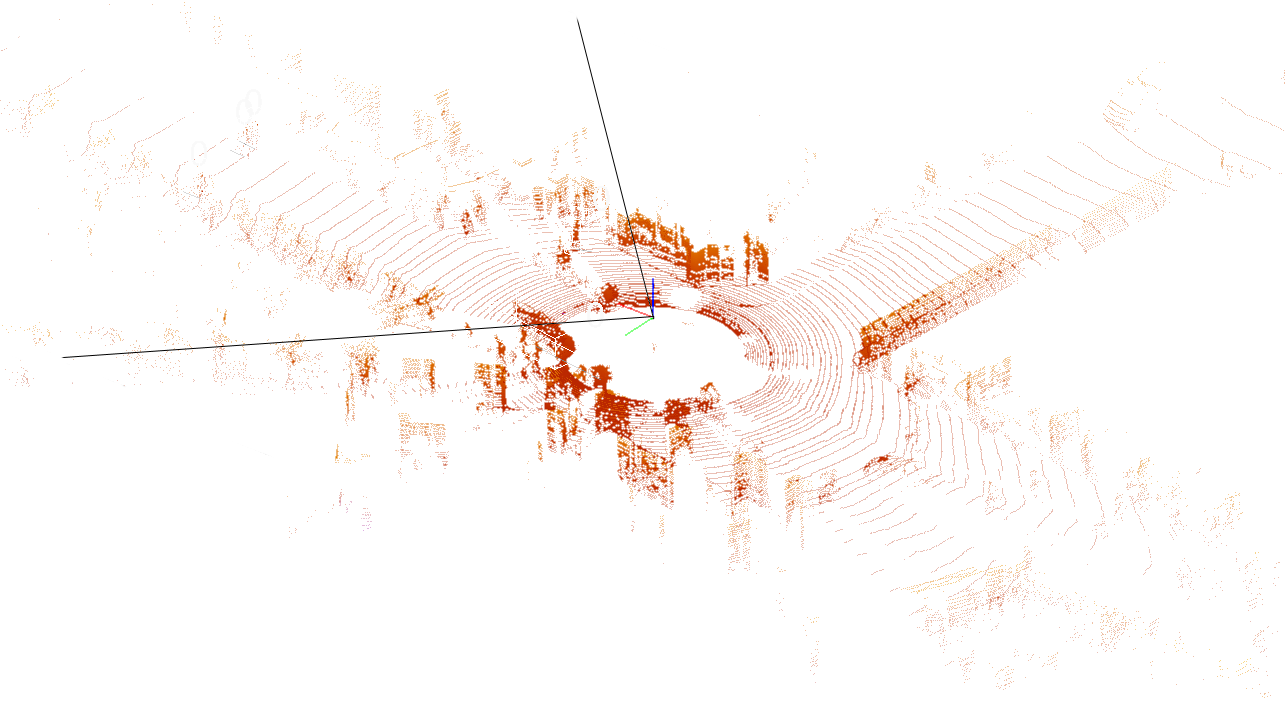
\includegraphics[width=0.8\linewidth]{../media/objdet_lidar_BEV_000015_light.png}
    \caption{Lidar pointcloud, alternate view. 3D bounding boxes are included as well as the horizontal field of view (angled lines leading away from coordinate system origin). Index 000015}
    \label{objdet_lidar_sample}
\end{figure}

\def \DEG{$^{\circ}$} % Don't want to import extra package for no reason right now.

\begin{table}[H]
	\centering
	\caption{KITTI object detection sample label from a given scene. Index 000015}
	\footnotesize
\begin{tabular}{|c|c|c|c|c|c|c|}
	\hline
	Class & Trun & Occl & Obs  & BBx1  & BBy1   & BBx2  \\
	\hline
	Car   & 0.89       & 0         & 2.29 & 0.00  & 194.70 & 414.71 \\
	\hline
\end{tabular}
\begin{tabular}{|c|c|c|c|c|c|c|c|}
	\hline
	BBy2   & HT   & WD   & DP   & Xc    & Yc   & Zc   & Roty \\
	\hline
	373.00 & 1.57 & 1.67 & 4.14 & -2.75 & 1.70 & 4.10 & 1.72 \\
	\hline
\end{tabular}
\label{kitti_label_sample}
\end{table}

In order to better understand the meaning of each value, each dataset provides a ``development kit" that contains a ``readme.txt" file. In the object detection devkit, the following text reproduced in Figure \ref{kitti_devkit_info}. Some of the names are different than what is used, but the order and purpose are identical.

\begin{figure}[ht] %h=here,t=top,b=bottom,H=exactlyHere
	\setstretch{0.8} % want code to be nice and compact
	% note: optional line numbers argument
	\small
	\begin{lstlisting}[language=tex]
Ct.  Name         Description
----------------------------------------------------------------------------
1    type         Describes the type of object: `Car', `Van', `Truck',
                      `Pedestrian', `Person_sitting', `Cyclist', `Tram',
                      `Misc' or `DontCare'
1    truncated    Float from 0 (non-truncated) to 1 (truncated), where
                      truncated refers to the object leaving image boundaries
1    occluded     Integer (0,1,2,3) indicating occlusion state:
                      0 = fully visible, 1 = partly occluded
                      2 = largely occluded, 3 = unknown
1    alpha        Observation angle of object, ranging [-pi..pi]
4    bbox         2D bounding box of object in the image (0-based index):
                      contains left, top, right, bottom pixel coordinates
3    dimensions   3D object dimensions: height, width, length (in meters)
3    location     3D object location x,y,z in camera coordinates (in meters)
1    rotation_y   Rotation ry around Y-axis in camera coordinates [-pi..pi]
1    score        Only for results: Float, indicating confidence in
                      detection, needed for p/r curves, higher is better.
	\end{lstlisting}
	\onehalfspacing % set line spacing back to normal
	\caption{Original text from readme.txt file of devkit\_object resources. The columns are: Ct. (``count"), Name (of value), and Description.}
	\label{kitti_devkit_info} % label goes last
\end{figure}

Beyond a few samples of the dataset, some statistics about the dataset can be found in both the accompanying paper as well as by looking through the dataset itself. From the original 2012 paper, \cite{geiger_are_2012} provided a subfigure of the class count across both training and validation data, reproduced below in Figure \ref{kitti_graph_objectcount}. When observing only the training data, the count of each class can be described. A quick summary of each value across all labels in the training dataset is given below in Table \ref{kitti_label_stats}. Note that the min/max range ignores the DontCare class and its values, such as -1000 for $z_c$.

\begin{figure}[H]
	\centering
	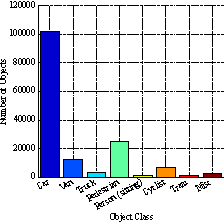
\includegraphics[width=0.4\textwidth]{../media/kitti_graph_objectcount.pdf}
	\caption{Object class count in KITTI object detection dataset, reproduced from \cite{geiger_are_2012}.}
	\label{kitti_graph_objectcount}
\end{figure}

\begin{table}[H]
	\centering
	\caption{KITTI dataset label statistics. Each numbered value's minimum and max values are given. Variables xc, yc, and zc are distance to the bounding box center of mass, and pixel values are given to sub-pixel accuracy.}
	\footnotesize
	\begin{tabular}{|c|c|c|c|c|}%
		\hline
		\bfseries Name & \bfseries DataType & \bfseries Unit & \bfseries min & \bfseries max % specify table head
		\csvreader[head to column names]{../media/kitti_label_stats.csv}{}% use head of csv as column names
		{\\\hline\csvcoli&\csvcolii&\csvcoliii&\csvcoliv&\csvcolv} % specify your columns here
		\\\hline
	\end{tabular}
	\label{kitti_label_stats}
\end{table}

The final bit of interesting statistical information may be found by counting the number of instances of each class. This is already provided by \cite{geiger_are_2012}, but in verifying the values provided only in the training data the exact number of instances of each class are listed below in Table \ref{kitti_class_stats}.

\begin{table}[H]
	\centering
	\caption{KITTI object detection class count. Semi-automatically counted through only labeled training data.}
    \footnotesize 
	\begin{tabular}{|c|c|c|c|c|c|c|c|c|}
		\hline
		Class & Car   & Pedestrian & Van  & Cyclist & Truck & Misc & Tram & Person\_sitting \\ \hline
		Count & 28742 & 4487       & 2914 & 1627    & 1094  & 973  & 511  & 222             \\ \hline
	\end{tabular}
	\label{kitti_class_stats}
\end{table}


\subsection{Evaluation Difficulty Levels}
One of the last but certainly not least important aspects of the KITTI dataset is the difficulty rating system. The KITTI dataset certainly has a variety of scenes and training data, but it also allows scoring to be performed on three difficulty levels, defined as follow:

\begin{enumerate}\itemsep=-0.6em
	\item Easy: 40 pixel min bbox height, max  level: Fully visible (0), max truncation: 15\%
	\item Moderate: 25 px minimum bbox height, max occlusion level: 1, max truncation: 30\%
	\item Hard: 25 px min bbox height, max occlusion level: 2, max truncation: 50\%
\end{enumerate}

Naturally, the ``Easy" difficulty typically earns a higher AP score than ``Moderate" (or ``Medium"), and ``Moderate" in turn typically yields a higher AP score than ``Hard". The official final score that a network receives when submitted to the KITTI Leaderboard is the ``Moderate" mean AP score. This paper specifically deals with the ``Car" class, so we may be able to better understand how these difficulties affect other parameters. Specifically related to the ``Car" class, 3D bounding box is considered a detection at 70\% overlap with a ground truth. The other two classes, ``Pedestrian" and ``Cyclist", only require an overlap of 50\%. The remaining other classes are not typically included in evaluation and scoring.

In the paper \cite{wang_pseudo-lidar_2019}, the ``Easy" evaluation for the ``Car" class is said to test on car labels located mostly within 30m of the ego vehicle, which was also claimed by another group, \cite{yang_pixor:_2018}. This was verified, and it is shown below in Figure \ref{kitti_labels_easyCar}.

\begin{figure}[H]
	\centering
	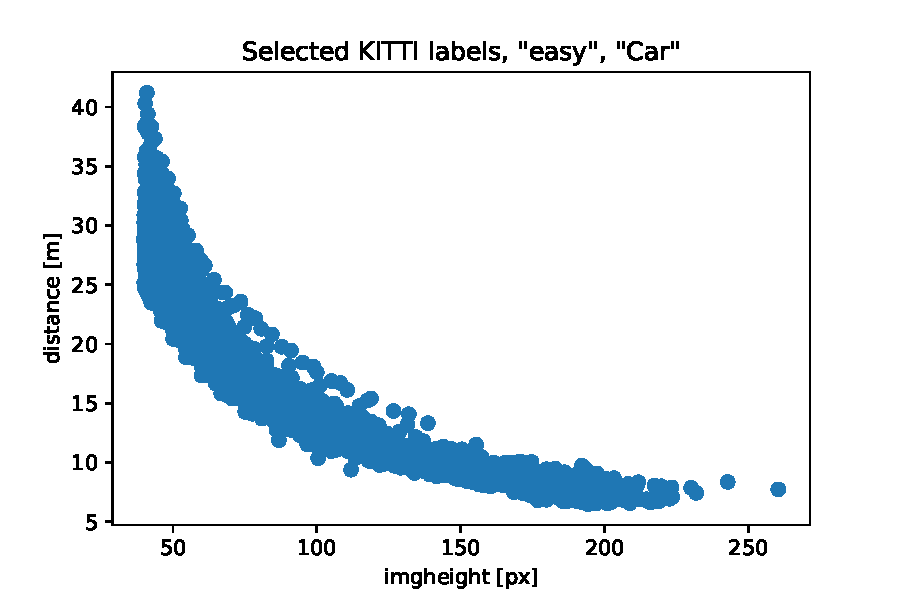
\includegraphics[width=0.6\textwidth]{../media/kitti_labels_easyCar.pdf}
	\caption{Filtered set of labeled training data containing only labels with the ``Car" class and those which are defined as ``Easy" difficulty. Just over 3\% of these filtered labels are beyond 30m. An interesting observation that may be made from the pixel height / distance relationship is that they are inversely correlated.}
	\label{kitti_labels_easyCar}
\end{figure}


%\newpage
%\section{KJG Checklist}
%
%things to ensure are in the report before you're done (completed items are commented out): 
%\begin{itemize} \itemsep=-0.7em
%% \item reformat general chapters to intro (incl. related work), topic1 (psmnet \& reconstruction), topic2 (fpnet), experiments, and conclusion
%% \item move performance metrics to "experiments" and leave examples as appendices
%% \item move 3D reconstruction to topic1 section
%\item change out the graphic about quadratic error (Figure 1.2?)
%\item make ertel corrections
%\item better clarify the steps of generating a pr curve
%\item complete the presentation
%\item fill out subsection related work: fpnet
%\item fill out subsection related work: stereo 3D object det
%\item fill out subsection "PSMnet and reconstruction"
%\begin{itemize} \itemsep=-0.6em 
%	\item understand \& explain spatial pyramid pooling "modules"
%	\item understand \& explain stacked hourglass "modules"
%	\item explain 3D reconstruction
%\end{itemize}
%\item fill out subsection fpnet with stereo 2 (psmstar)
%\item ensure that epipolar triangle figure has u_0 instead of x_0.
%\item create proper images / figures / tables for each section
%\item explain that only the car class is being focused on, because of it's high frequency of appearance in the kitti dataset and being a somewhat simpler target than a pedestrian.
%\item cite everything correctly
%\item no more 'xx' items
%\item need to rewrite areas around citations
%\item no missing references, has a question mark "?"
%\item USE AMERICAN NOTATION, COMMAS AND PERIODS WHERE YOU'RE USED TO.
%\item ensure double quotes are properly marked with ``, not "
%\item replace (where possible) png images with high res pdf images. ex: figure 4.1 on different outcomes
%\item ensure using consistent naming for SPCLnet everywhere
%
%\end{itemize}

